\documentclass{report}
\usepackage{graphicx}
\usepackage{amsmath}
\usepackage{rotating}
\setlength{\parskip}{1em}
\renewcommand{\abstractname}{Summary}
\usepackage{nomencl}
\makenomenclature

\begin{document}
\begin{titlepage}
	\centering
	
\includegraphics[width=0.25\textwidth]{graphics/logo}\par\vspace{1cm}
	{\scshape\LARGE University of Bath \par}
	\vspace{1cm}
	{\scshape\Large Final year project\par}
	\vspace{1cm}
	{\huge\bfseries Wave energy converter power increase through active control: Fixed Gains\par}
	\vspace{2cm}
	{\Large\itshape Carl Selig\par}
	\vfill
	supervised by\par
	Dr.~Andrew \textsc{Hillis}\par
	assessed by\par
	Dr.~Joseph \textsc{Flynn}

	\vfill

% Bottom of the page
	{\large \today\par}
\end{titlepage}

\begin{abstract}
Lorem ipsum
\end{abstract}
\section*{Acknowledgements}
Hi mum x
\tableofcontents
\listoffigures
\listoftables

\mbox{}

\nomenclature{$WEC$}{Wave Energy Converter}
\nomenclature{$IMC$}{Internal Model Control}
\nomenclature{$DOF$}{Degree(s) of Freedom}

\printnomenclature

\chapter{Introduction}
This report seeks to present the results of the research project conducted by the Author as well as the means to reproduce them. The project is part of a larger research effort to increase the power generation of Wave Energy Converters (WECs) through control system design. It is hoped that improved power generation will increase the commercial viability of the field. Wave power is already considered a viable energy source for the UK \cite{carbonTrust} but has not seen significant implementation at the time of writing \cite{europeanMarineEnergyCenter}.

Wave power refers to a group of technologies that harvest energy from sea waves. It is distinct from Tidal power. Wave power is relevant as a renewable energy source that has advantages over other sources such as solar and wind. Most notably, it constantly produces a base amount of power; can be used along most coastlines; and has a low initial expenditure. \cite{carbonTrust}

The WEC examined in this project is modelled after the Wave Sub device developed by Marine Power Systems\cite{waveSub}. \ref{fig:waveSub} shows a published graphic\cite{waveSub} of this device against the modelled WEC. It was chosen as a generic example of a multi-DOF WEC. The Carbon Trust describes multi-DOF WECs as being of particular interest to UK energy infrastructure due to their increased potential for energy capture over single DOF WECs \cite{carbonTrust}.



\begin{figure}
\centering
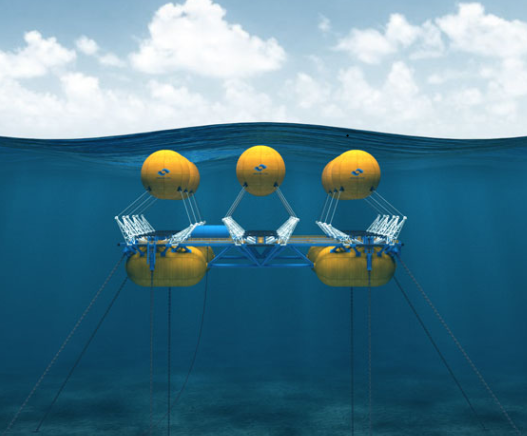
\includegraphics[height=0.4\textwidth]{graphics/waveSub}
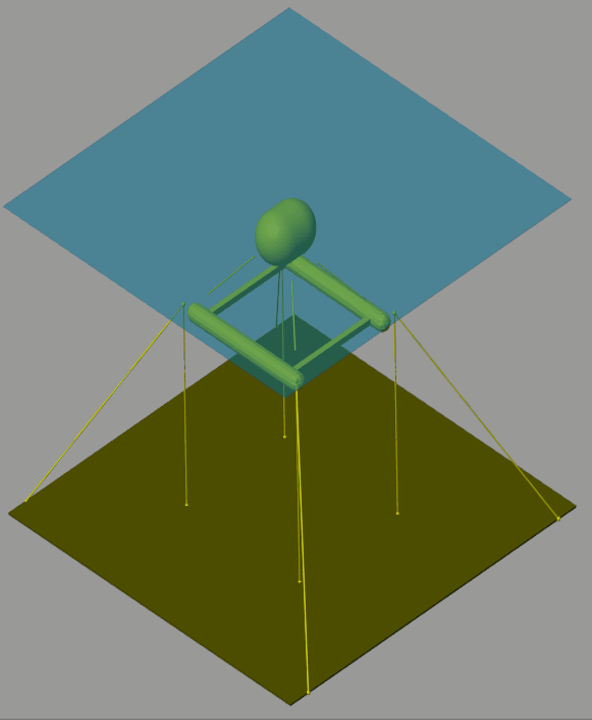
\includegraphics[height=0.4\textwidth]{graphics/wecSimFloat}
\label{fig:waveSub}
\caption{A graphic of an array of 9 WaveSub devices(left)\cite{waveSub} versus the modelled WEC(right). Note that cable arms exist in the left figure but are absent in the right due to divergent design.}
\end{figure}

The model shown in \ref{fig:waveSub}  was created using a simulation environment known as wecSim\cite{wecSim}.
 
 the adaptation of a "Simple and Effective" control strategy initially proposed by JV Ringwood \cite{ringwood} from 1 dime


Figure 3 A graphic of an array of 9 WaveSub devices. (Marine Power Systems, 2019). In this project the PTOs will be modelled as cable-drums rather than the arms shown. A pre-existing simulation environment known as WECSim has been made available by Dr. Andrew Hillis. This simulation was used in various works by Dr. Hillis to compare the power extraction of a Model Predictive Control (MPC) scheme to an, “Optimally tuned, passively damped” system (Hillis, To Appear) (Hillis, et al., To Appear). This approach will be used in this project to assess control system performance. Many control schemes have been used to increase the power absorption of the WaveSub device and other WECs such as floating-point absorbers (Abdelkhalik, et al., 2017). Of note is a scheme known as, “Simple and Effective,” control proposed by John Ringwood and Francesco Fusco (Fusco \& Ringwood, 2013). They claim that this scheme approaches the effectiveness of an MPC scheme whilst being both simpler and more robust. The claim of having advantages over MPC is attractive since MPC is considered an industrial standard due to its ubiquity in digital controllers (Gorinevsky, 2005). MPC schemes are straightforward to implement and can optimise for the present time period whilst also considering future input. They are understood well enough that they can often be redesigned “on the fly,” (Gorinevsky, 2005). Both control schemes rely on a model of the system. In the case of Simple and Effective control the system uses an analytical model to predict Wave Excitation Force. This is taken as an input, then passed to an Extended Kalman Filter and an adaptive law based on wave peak frequency to evolve an optimal velocity trajectory. The control system then subjects the WEC PTO to Proportional-Integral control in order that the prime mover tracks the velocity trajectory. The block-diagram for this scheme is shown in Figure 4. 

Figure 4: Reproduction of figure 3 from “A Simple and Effective Real-Time Controller for Wave Energy Converters,” (Fusco \& Ringwood, 2013). Shown are the estimated Wave Excitation Force input, $f_ex$ (t); the Extended Kalman Filter (EKF) and Adaptive law implementation, and finally the Proportional Integral control loop. Wave Excitation Force is estimated as sinusoidal. The Simple and Effective control scheme therefore offers a significant advantage over more computationally intensive methods, including the supposedly cheap MPC. However, these results have only been shown to be true for WECs that are constrained to 1 axis (heave). In unpublished work, Hillis has implemented this control scheme in a 6 Degrees-Of-Freedom (6DOF) system using Internal Model Control. He has observed that the float drifts from its home position over time, eventually violating the device’s constraints. 




\chapter{Literature Review}
The modern concept of wave power was first proposed in 1974 by Stephen Salter in the form of the self-styled Salter duck \cite{salterDuck}. This device was proposed as an alternative to oil during the 1973 Oil Crisis in the UK. As shown in Figure 1 the Salter duck generates power by having its vane (beak) bobbed by incoming waves.

\begin{figure}
\centering
\label{fig:duck}
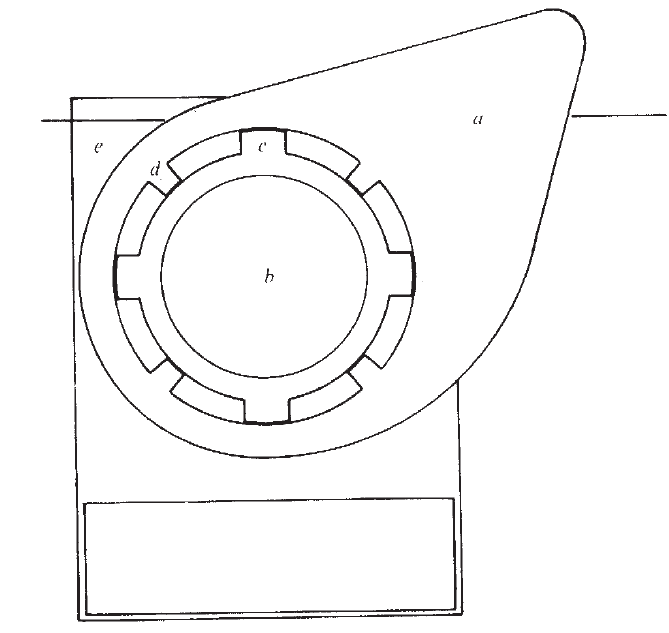
\includegraphics[scale=0.25]{graphics/duck}
\caption{A reproduction of a figure from “Wave Power,”\cite{salterDuck}. “a. vane; b, a hollow cylindrical member; c, paraxial ridges; d, inward facing ridges on the vane; e, vertical fin between this vane and the next.”}
\end{figure}

Salter is considered a foundational figure in the sector [REF]. By his own account in, "Wave Power: Nostalgic Ramblings, future hopes, and heretical suggestions" \cite{salterRamble} the early years of wave power are the history of him and his colleagues.

Salter received funding from the UK Department of Energy to set up a laboratory in Edinburgh. Wave power also garnered interest from other British academics, notably David Evans in Bristol who invented the Bristol Cylinder. (Evans, et al., 1979).
Evans also developed theories on the hydrodynamics and efficiency of WECs under idealised conditions (Evans, 1976). His work concerns a one-dimensional scenario where waves are modelled as perfect sinusoids that meet the WEC at right angles. This is not the case in nature and thus his claim that 100% extraction of wave energy is possible has never been produced in practice.
Unfortunately, with the conclusion of the Oil Crisis, Salter and Evans found it increasingly difficult to secure funding for their research and none of their devices have been brought to market. In his Review article titled, “Wave energy: Nostalgic Ramblings, future hopes and heretical suggestions,” Salter blames pressure from the nuclear sector and “others [who] set out to destroy what they saw to be a threat,” (Salter, 2016). He then goes on to explain that whilst WECs were initially billed as very simple the reality is significantly more complex.
At the time of writing there have been two WEC projects in the UK that have reached commercialisation. Pelamis from Pelamis Wave Power and Oyster from Aquamarine Systems. (The European Marine Energy Center Ltd., 2019). Figure 2 shows these devices as they were installed. Pelamis 1 was installed in 2004 and became the first WEC to provide power to a National Grid. Pelamis 2 became the first WEC to be purchased by a utility company in 2009. Oyster was installed in 2012. Both devices provided power to the National Grid over the course of their lifetimes.

  
Figure 2: Pelamis 2 [Top] and Oyster [Bottom] as installed at the Billia Croo wave test site in Orkney, Scotland. (The European Marine Energy Center Ltd., 2019)
Similarly to Salter and Evans, both organisations found it difficult to secure funding after their initial funding lapsed. Both companies went into administration a few years after the installation of their WECs. This appears to be a recurring problem in the industry as there have been many other promising WEC projects that have failed to find investors. Examples include Corpower Ocean and Seatricity (The European Marine Energy Center Ltd., 2019).

It appears previous WECs were not economically viable as no WEC project to date has consistently made profit. Investors have also proven unreliable long-term. Barring global economic change there is a need to make WECs more profitable if they are to become a national power source.

One way of increasing the viability of a WEC is to use a control system. By taking the current Wave Excitation Force as an input the power extraction of a WEC can be optimised. In this project an in-development WEC known as WaveSub is used to investigate  the effectiveness of fixed gain control schemes for power optimisation.
The WaveSub device consists of a submerged cylindrical float tethered to an underwater platform via 4 cables. The cables drive Power Take Offs (PTOs) that can extract energy from the motion of the float relative to the platform. (Marine Power Systems, 2019)



Works from the 2019 EWTEC conference which use alternative tracking control do not exhibit this drift. The cause of the drift is unknown and represents a novel research subject. There has been comparatively little work on 6DOF WECs compared to planar devices like the Salter duck and Bristol Cylinder. This project will seek to replicate the drift result and will investigate its cause. Ideally the drift could be rectified without the need for additional control loops, retaining the computational simplicity of the scheme. Estimating the Wave Excitation Force becomes more complex in 6DOF. It is necessary to consider all the forces and Torques acting on the float. This can be represented as a 6×1 vector known as a Wrench, making it the Wave Excitation Wrench.

It may be possible to adapt existing work on Heave only WECs into this format. Nguyen and Tona have presented a detailed account on two methods of Wave Excitation Force estimation (Nguyen \& Tona, 2018). Alternately there is a wealth of research available on semi-analytical or computational methods. M. Folley’s book, “Numerical Modelling of Wave Energy Converters” (Folley, 2016) is a modern collection of these methods.

Finally, it is necessary to construct a state-vector for the system. In heave only WECs this is a single variable. For 6DOF WECs the state vector can be represented in the form of a 6×6 homogeneous matrix transform. There are two ways to derive this transform which are referred to as the active view and the passive view. (Merlet, 2006)
 The passive view has been successfully used in prior research (Hillis, et al., To Appear) however the active view may merit investigation. Since the WaveSub device is a class of cable robot its equations of motion can be derived using Screw Theory.
Given the forces on the float as a Wrench and its state as a Homogeneous Transform it is easy to write the equations of motion of the body. It is considerably harder to find solutions to the equations of motion since according to (Merlet, 2006) the space of all rigid body displacements in this or any equivalent system is non-linear (manifold).
Screw theory proposes to linearise these equations of motion by using the tangent space of all rigid body motions of the system. That is, by considering small displacements over small time periods a (virtual) velocity twist is constructed. The space of all velocity twists is linear.
Multiplying the velocity screw by the body’s inertia matrix (calculated from physical parameters) gives the momentum wrench. The equations of motion for the system can then be described as:

d/dt Momentum Wrench=Wave Excitation Wrench
This is now a non-linear first order differential equation which may be solved by numerical methods. Analytical solutions are usually impossible and certainly not practical for a digital controller.
J.P. Merlet’s book “Parallel Robots,” (Merlet, 2006) offers a comprehensive explanation of modelling cable robots, and J. Selig’s book, “Geometrical fundamentals of Robotics,” explains how to apply Screw Theory to parallel robots.

\chapter{Aims and Objectives}
The aims of this projected are phrased as 3 research questions.
\begin{enumerate}
\item{Does a drift problem occur if Ringwood's Simple and Effective Control strategy is adapted for planar motion?}
\item{If the drift problem exists, can it be resolved?}
\item{How much power does this implementation generate compared to an optimally tuned, passively damped system?}
\end{enumerate}

To answer these questions, it was necessary to achieve the following objectives.

\chapter{Research Methodology}

\chapter{Simple and Effective Control}
Simple and effective control refers to a strategy presented by Fusco and Ringwood in their paper, "A simple and effective real-time controller for wave energy converters,"\cite{ringwood}. This strategy was designed for a 1-DOF WEC, however the WaveSub device considered in this project is a 6-DOF device. This complicates the implementation of simple and effective control. Simplifying assumptions were made which are described in Section \ref{section: assumptions}. The most important of these is the assumption that the WaveSub device behaves as a planar device, and that only surge and heave motions are controlled. Therefore the control strategy need only be adapted for 2 DOF, rather than 6.

Figure \ref{fig:fullControl} shows the full implementation of the control strategy in the Simulink environment. This chapter will detail each component in sufficient detail that the reader may re-create the system.

\begin{sidewaysfigure}[h]
\centering
\label{fig:fullControl}
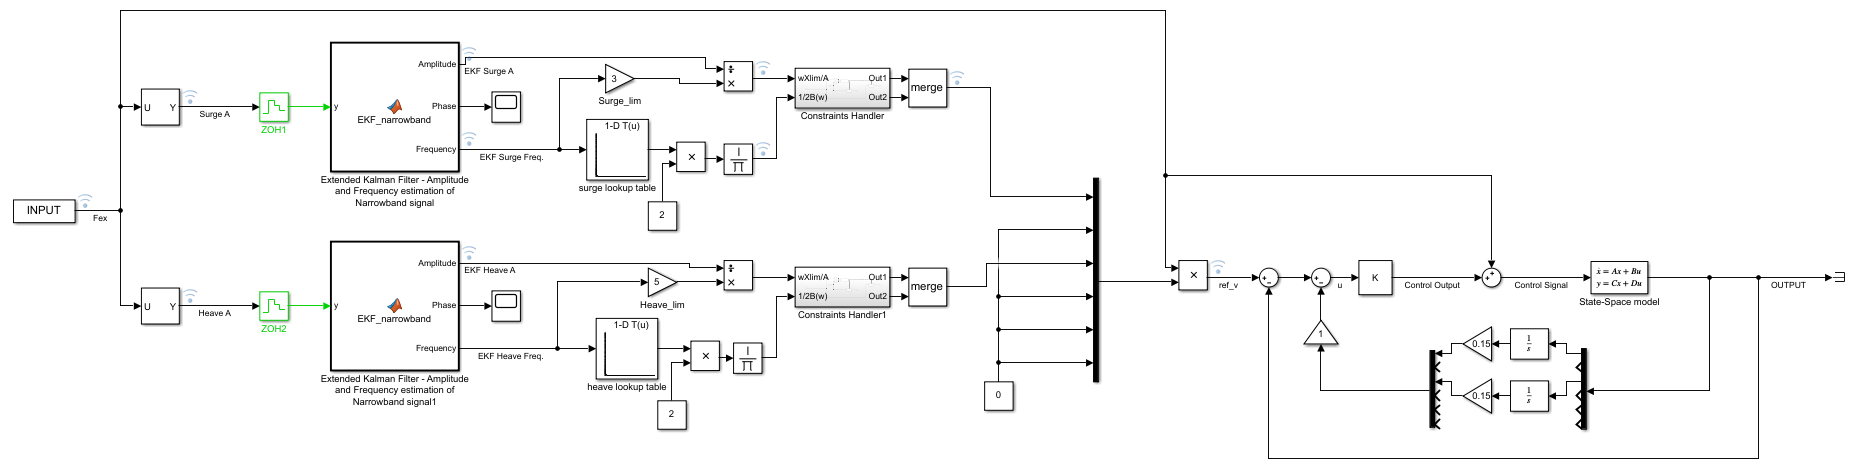
\includegraphics[scale=0.5]{graphics/fullControlSystem}
\caption{The full implementation of simple and Effective Control for the WaveSub device.}
\end{sidewaysfigure}


%Fusco and Ringwood report that their control strategy provides, "levels of power capture close to MPC in most sea states... without the need of predictions and the solution of an optimization[sic] problem in real time."\cite{ringwood}. %Move this to another section.


\section{Simplifying assumptions}
\label{section: assumptions}

Sea states are modelled as being irregular, meaning that they are the sum of many simple harmonic (regular) waves with a variety of amplitudes and frequencies. Real life waves can be described this way via Fourier analysis. However, since infinite sums cannot be realised by a real-time controller some approximation is necessary. Moreover, the waves used in the simulation are generated, rather than being recordings of real waves.

The energy distribution within the generated irregular waves is modelled using an empirical relationship known as the Pierson-Moskowitz spectrum as described in "A proposed spectral form for fully developed wind seas based on the similarity theory of S. A. Kitaigorodskii," by Pierson and Moskowitz\cite{OGPM}. This spectrum relates wave frequency and energy distribution and is based on the assumption that sea waves are in equilibrium with the wind. A 2003 review paper using modern wave data reaffirmed that "for the chosen data only... [the spectrum] provides statistically robust relations."\cite{PMReview}


\section{Internal Model Control}
Internal Model Control is 

\section{Discrete State Space Model}

\section{Inverting the discrete state-space model}
To implement Internal Model Control it is necessary to create both a model of the plant and an inverse of that model. The plant model is provided from [ANDY’S EWTEC PAPER] in the form of a state-space model. Creating a robust inverse of this model is a task for this project.

One potential approach is to convert the state-space system into a system of transfer functions. In this case the inverse is simply the reciprocal of the transfer function. This method is complicated by the fact that the plant is a 6x6 MIMO system. Generating corresponding transfer functions using inbuilt MATLAB methods results in 36 very high order transfer functions. Problems with this include:
\begin{itemize}
	\item{Over-fitting to the model}
	\item{Improper after being inverted, requiring a filter to be realisable}
	\item{Only practical to consider a maximum of 6 transfer functions, ignoring cross terms. (2 in practice)}
\end{itemize}


The Massey-Sain algorithm is an alternate method for creating a real-time inverse of a state space system. It was first presented in IEEE Transactions on Automatic Control, vol.14, 1969. Later it was summarised in a lecture given by Sundaram at the University of Illinois at Urbana-Champaign. The following derivation is paraphrased from Sundaram's lecture.

First it is necessary to convert the continuous time state-space model to a discrete time model. This is achieved using the ‘c2d’ function in MATLAB. Using discrete time also prevents any errors caused by the numerical methods of the Simulink solver.

First it is necessary to test whether or not the system is invertible. All discrete-time state space systems are of the form:
\begin{equation}
	x(t+1)=Ax(t)+Bu(t)
\end{equation}
\begin{equation}
	y(t)=Cx(t)+Du(t)
\end{equation}

Where x is the state vector; y is the output vector; u is the input vector; A is the state matrix; B is the input matrix; C is the output matrix; and D is the disturbance matrix.

For our system there is no disturbance input and so D is the zero matrix. It will not be shown in further equations.

Paraphrasing from Sundaram:
“A system has an inverse with delay $L$ if $u(t)$ can be uniquely determined from $y(t),y(t+1),…y(t+L)$  (and perhaps $x(t)$)”

So, we need to find the lowest possible value of L. It is possible to express later time-steps in terms of the current time step via substitution.
\[					%delimiters for 'displaymath' environment, no numbering.
	y(t+1)=Cx(t+1)
\]

Substituting equation 1:
\[
	y(t+1)= Ax(t)+Bu(t)
\]

This can be iterated for arbitrarily large timesteps. It can also be represented in a matrix format:

\[
	\begin{bmatrix}
		y(t)   \\
		y(t+1) \\
		y(t+2) \\
		\vdots \\
		y(t+L)
	\end{bmatrix}
	=
	\begin{bmatrix}
		C   \\
		CA  \\
		CA^2\\
		\vdots\\
		CA^L
	\end{bmatrix}
	x(t) +
	\left[
	\begin{array}{c|cccc}			%Have to use 'array' to do partitions
	0&0&0&\hdots&0						\\
	CB&0&0&\hdots&0						\\
	CAB&CB&0&\hdots&0					\\
	\vdots&\vdots&\vdots&\ddots&\vdots	\\
	CA^{L-1}B & CA^{L-2}B & CA^{L-3}B & \hdots & 0
	\end{array}
	\right]
	\left[
	\begin{array}{c}
		u(t)		\\
		\hline
		u(t+1)		\\
		u(t+2)		\\
		\vdots		\\
		u(t+L)
	\end{array}
	\right]
\]
\begin{equation}
=Y_{(t,L)} = O_Lx(t)+M_L U_{(t,L)}
\end{equation}

Where $O_L$ is analogous to the Observability of the system, and $M_L$ to its Measurability. The partitions show that $M_L$ contains the smaller matrix $M_{L-1}$. This can be iterated for all versions of $M_L$ down to $M_0$.

Massey \& Sain's theorem asserts that if the rank of $M_L$ minus the rank of $M_{L-1}$ is equal to the number of columns $'m'$ of $M_{L-1}$ then there exists a matrix $\mathcal{K}$ such that
\[
\mathcal{K}M_L =
\left[
\begin{array}{c|c}
I_m & 0
\end{array}
\right]
\]
Multiplying equation 3 by $\mathcal{K}$:
\[
\mathcal{K}Y_{t,L} = \mathcal{K}O_Lx(t) + u(t)
\]
Hence the input $u(t)$ can be expressed in terms of the outputs $Y_{t,L}$

\begin{equation}
u(t) = -\mathcal{K}O_Lx(t) + \mathcal{K}Y_{t,L}
\end{equation}

Similarly the state vector at time $t+1$ can be found by substituting equation 4 into equation 1
\begin{equation}
x(t+1) = (A-B\mathcal{K}O_L)x(t) + B\mathcal{K}Y_{t,L}
\end{equation}

Equations 4 and 5 together represent the inverse State-space model.

The task is now to see if there exists a value of L for our system that will satisfy the Massey-Sain theorem. In the case that there are multiple viable values of L the smallest value is preferable as any inverse constructed with it will have the smallest possible delay.

In the case of our 6 input, 6 output system
\begin{itemize}
\item{$M_0$ is the $6\times6$ zero matrix. It has rank 0, and 6 columns(m=6).
}
\item{$M_1$ has the form
\[
\left[
\begin{array}{cc}
0	&	0	\\
CB	&	0	\\
\end{array}
\right]
\]
where $CB$ is a full-rank $6\times6$ matrix, making the overall rank 6.
}
\end{itemize}

Therefore the system is invertible with $L=1$ since
\[
rank(M_1) - rank(M_0) = m_0
\]

As above the matrix $\mathcal{K}$ is formed by performing a pseudo-inverse of $M_1$ less the last 6 columns. This results in a $12\times6$ matrix. This is expected since
\[
Y_{t,L} = Y_{t,1} =
\begin{bmatrix}
y(t)	\\
y(t+1)
\end{bmatrix}
\]
so to find the inverse at the time-step $t+1$ the inverse system must be given both $y(t)$ and $y(t+1)$. since y is a $6\times1$ vector this makes $Y_{t,1}$ a $12\times1$ vector which matches the dimensions of $\mathcal{K}$.

The inverse is then constructed according to equations 4 and 5, and a one time-step delay is used to generate $y(t)$ at the timestep $t+1$.

This results in a robust inverse system. When used in the IMC loop it is able to perfectly track simple sinusoid input save for a delay of one time-step. It is hoped that this delay will be negligible for small time-steps.

\section{Adaptive Controller}

\section{Filtering Wave Excitation Force}

\section{Velocity Constraints}

\section{Integral Position control}

\chapter{Results}

\chapter{Discussion}

\chapter{Conclusions}

\section{Future Work}


%\begin{sidewaysfigure}[h]
%	\centering
%	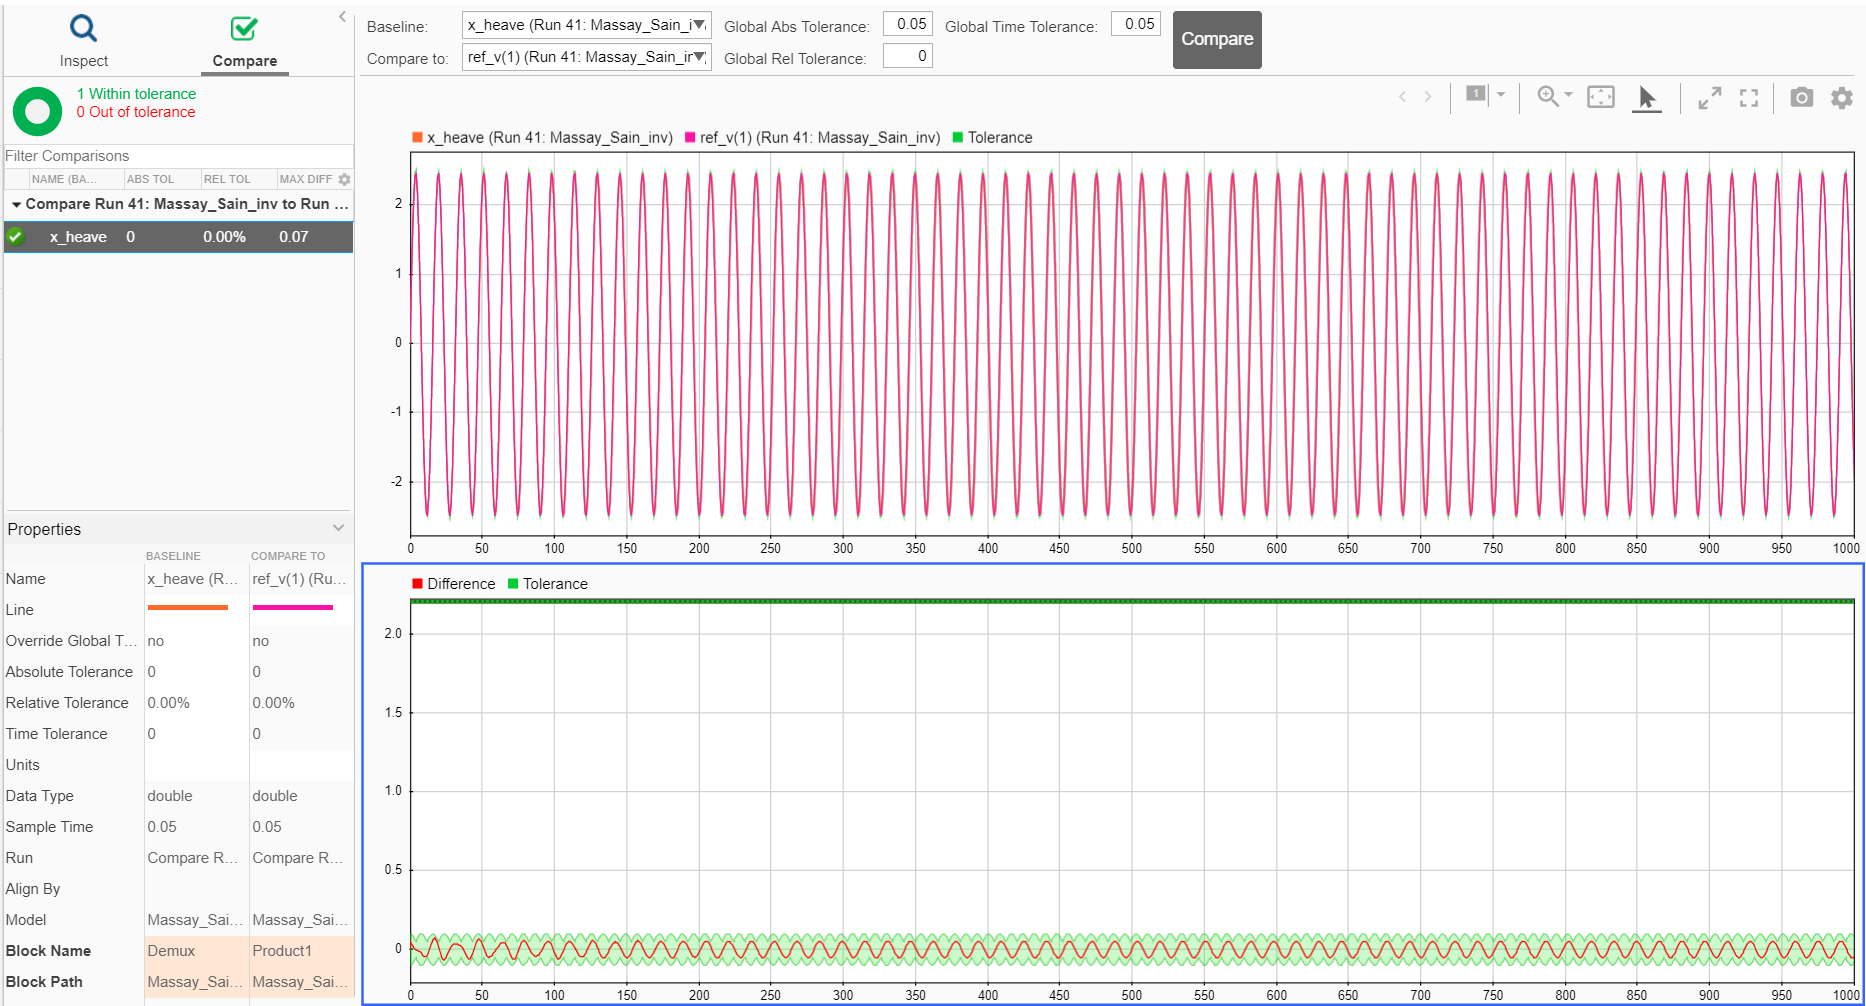
\includegraphics[scale=0.55]{heaveTracking}
%	\caption{A simulink data inspector comparison of the heave input and the output of the control loop. The input was a sinusoid with amplitude $10^6m$ and frequency $0.4rads^{-1}$. The time step was $0.05s$. The output matches the input with a global tolerance of $0.05 units$.}
%\end{sidewaysfigure}

\bibliography{bibliography}
\bibliographystyle{IEEEtran}
\end{document}